\documentclass[tikz,border=5pt]{standalone}
\usepackage{tikz}
\usepackage{amsmath}
\usetikzlibrary{arrows.meta,calc}
\definecolor{nebula}{HTML}{6366F1}
\definecolor{spark}{HTML}{14B8A6}
\definecolor{ink}{HTML}{334155}
\begin{document}
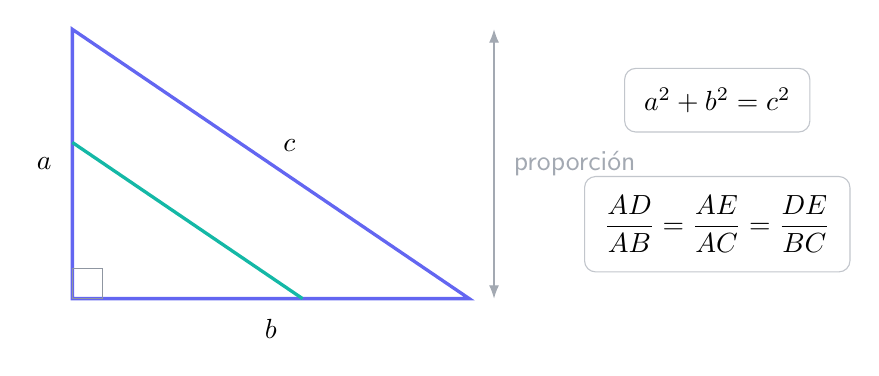
\begin{tikzpicture}[font=\sffamily,>=Latex,scale=.9]
  \coordinate (A) at (0,0); \coordinate (B) at (5.6,0); \coordinate (C) at (0,3.8);
  \draw[very thick,nebula] (A)--(B)--(C)--cycle;
  \draw[ink!55] (0,0) rectangle (.42,.42);
  \node[left=4pt] at (0,1.9) {$a$};
  \node[below=4pt] at (2.8,0) {$b$};
  \node[above right=1pt] at (2.8,1.9) {$c$};
  \coordinate (D) at ($(A)!.58!(B)$);
  \coordinate (E) at ($(A)!.58!(C)$);
  \draw[very thick,spark] (D)--(E);
  \draw[<->,ink!45] (5.95,0)--(5.95,3.8) node[midway,right=5pt,fill=white,inner sep=2pt] {proporción};
  \node[draw=ink!30,rounded corners=4pt,fill=white,inner sep=7pt] at (9.1,2.8)
    {$a^2+b^2=c^2$};
  \node[draw=ink!30,rounded corners=4pt,fill=white,inner sep=7pt] at (9.1,1.05)
    {$\dfrac{AD}{AB}=\dfrac{AE}{AC}=\dfrac{DE}{BC}$};
\end{tikzpicture}
\end{document}
